\chapter{Instrumentação Industrial}

A instrumentação é relativa aos equipamentos que obtem informações acerca do estado de um determinado processo industrial. Os chamados sensores e transdutores.

A definição de sensor e transdutor está longe de ser uma unanimidade. Do ponto de vista da instrumentação, define-se:
\begin{description}
  \item[Sensor] é um elemento que gera um sinal (normalmente elétrico) a partir de uma grandeza física (calor, luz, som pressãom etc).
  \item[Transdutor] é um dispositivo que converte um sinal de uma grandeza para outra.
\end{description}

De onde se tira que todo sensor é um transdutor, mas não o contrário. Em geral os sensores se utilizam de transdutores para converter uma grandeza específica para outra mais facilmente manipulável.

Outra classificação normalmente usada é a de sensores passivos ou ativos:
\begin{description}
  \item[Sensores ativos] geram um sinal de saída sem a necessidade de alimentação externa. Exemplos: termopar, célula fotoelétrica.
  \item[Sensores passivos] requerem uma entrada de energia para gerar um sinal de saída. Exemplos: Termoresistência, sensor capacitivo.
\end{description}

A maioria dos sensores industriais são passivos.

Outra classificação bastante útil é a de sensores discretos ou contínuos:

\begin{description}
  \item[Sensores discretos] geram uma saída discreta, normalmente binária -- do ponto de vista da saída elétrica agem como chaves e são comumente chamados de sensores.
  \item[Sensores contínuos] geram uma saída que varia continuamente em função da entrada. Pode ser composto por um único transdutor (um resistor por exemplo).
\end{description}

Um complicador é que alguns textos técnicos apresentam uma confusão de sensores e transdutores com sensores discretos (chamados simplesmente de sensores) ou contínuos (chamados erroneamente de transdutores). Portanto deve-se tomar cuidado com o significado destes termos.

\section{Sensores discretos}

Como citado, a maioria dos sensores discretos industriais são chaves elétricas. Neste caso diferenciam-se os sensores de contato, que são chaves eletromecânicas; os sensores de proximidade, que detectam a presença de algum objeto sem tocá-lo; e as chaves de processo.

\subsection{Sensores de contato}
Do ponto de vista da instrumentação, qualquer chave presente no nível 1 da pirâmide que gera sinais lidos no nível 2 realizam logicamente o mesmo tipo de função. Daí que se consideram como sensores de contato:
\begin{description}
  \item[Botoeiras] ou botões, acionados pelo operador do processo.
  \item[Chaves de fim de curso] que são acionadas mecanicamente por algo no processo.
\end{description}

As botoeiras podem ter diversos formatos e funções, vide a figura~\ref{fig:botoeiras}. Podem ser simples botões acionados apenas quando pressionados, interruptores de 3 estados, entre outros. Alguns botões de emergência são acionados quando apertados e só são desligados com o uso de uma chave. Também é comum botoeiras que energizam equipamentos poderem ser travadas na posição desligada com um cadeado. Isto permite que o manutentor trave o equipamento desenergizado enquanto efetua algum serviço.

\begin{figure}
  \centering
  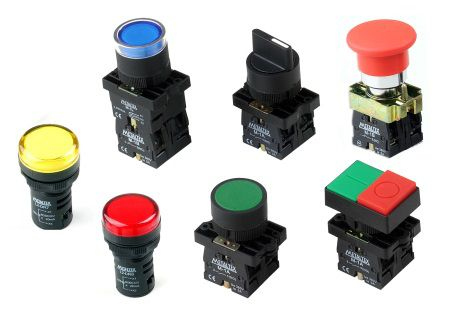
\includegraphics[width=0.6\textwidth]{figuras/botoeiras}
  \caption{Diversos tipos de botoeiras.}\label{fig:botoeiras}
\end{figure}

Chaves de fim de curso são chaves eletromecânicas feitas para serem acionadas por algum produto ou equipamento. São usadas para detectar, por exemplo, a passagem do material sendo processado por um determinado ponto, a posição final de movimentação de algum equipamento, entre outros. Normalmente é implementado como um botão com uma alavanca ou algum outro mecanismo na parte a ser acionada.

\begin{figure}
  \centering
  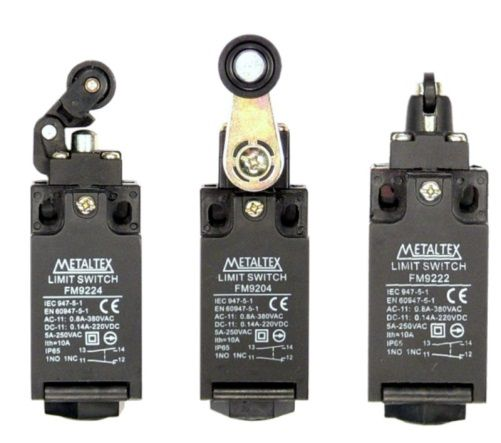
\includegraphics[width=0.6\textwidth]{figuras/fim-de-curso}
  \caption{Exemplos de chaves de fim de curso.}\label{fig:fim-de-curso}
\end{figure}

As chaves eletromecânicas são relativamente baratas, de uma tecnologia já bem amadurecida e são imunes a interferências eletromagnéticas, porém o movimento a que são submetidas gera desgaste, o que faz com que sua vida útil seja reduzida. Além disso, necessitam do contato com o alvo para ser acionadas, o que pode ser inviável em alguns casos, e tem um tempo de resposta da ordem de milisegundos, que pode ser lento demais para algumas aplicações.

\subsection{Sensores de proximidade}

 Existem diversos princípios físicos que podem e são usados para detectar a proximidade de algum material. Estes são chamados de sensores de proximidade e normalmente são aplicados quando se tem algum impedimento ao uso de chaves eletromecânicas.

Para vários casos, é comum o uso de um encapsulamento em formato de rosca, como visto na figura . Isto faz com que vários sensores de proximidade se pareçam, mesmo que usem princípios físicos diferentes.

\begin{figure}
  \centering
  {\Huge FALTA ESTA FIGURA!}%\includegraphics[width=0.6\textwidth]{figuras/proximidade}
  \caption{Encapsulamentos comuns para sensores de proximidade.}\label{fig:proximidade}
\end{figure}

\subsubsection{Indutivo}
\label{subs:Indutivo}
O sensor indutivo conta com uma bobina na sua extremidade sensora, que gera um campo magnético variável na sua frente. A frequência deste campo magnético depende da própria indutância desta bobina, que por sua vez depende do que estiver na frente do sensor.

Um alvo que esteja na frente deste sensor pode alterar esta indutância por 2 efeitos: se for um condutor, gerará um campo magnético contrário, aumentando a indutância; se for ferroelétrico, concentrará o campo magnético, também aumentando a indutância. Este segundo efeito é maior que o primeiro, o que faz com que este sensor responda melhor a ferro do que a cobre, mesmo com o cobre sendo melhor condutor que o ferro.

A distância que um sensor indutivo consegue detectar um alvo de ferro na sua frente é chamada de \textbf{distância sensora nominal}. Para outros materiais esta distância diminui e para materiais não condutoros e sem propriedades magnéticas ela cai a zero. A figura \ref{fig:distancia_sensora} mostra a variação da distância sensora de sensores indutivos e capacitivos para diferentes materiais.

\begin{figure}
  \centering
  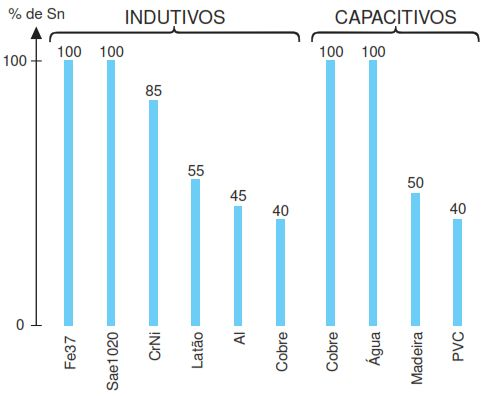
\includegraphics[width=0.6\textwidth]{figuras/distancia_sensora}
  \caption{Variação da distância sensora de sensores indutivos e capacitivos para diferentes tipos de material.}\label{fig:distancia_sensora}
\end{figure}

Além da limitação da distância que pode ser usado e da limitação do material do alvo, sensores indutivos estão sujeitos a interferências eletromagnéticas, que podem gerar falsas detecções.

\subsubsection{Capacitivo}
\label{subs:Capacitivo}

Sensores capacitivos usam um circuito oscilador (basicamente o mesmo de sensores indutivos) para detectar a variação da capacitância entre duas placas metálicas na sua ponta. Esta capacitância varia se o alvo tiver uma constante dielétrica diferente que a do ar. Funciona muito bem para água e cobre (que tem uma constante dielétrica 80 vezes maior que o ar). Praticamente não responde para ferro aço e alumínio.

Pela fraca sensibilidade a papel e plástico, pode detectar a presença de alguns objetos dentro da embalagem. Pela alta sensibilidade à água, é muito usado para detecção de nível. Também é sensível à interferência eletromagnética, embora menos que o indutivo.

\subsubsection{Ultrassônico}
\label{subs:Ultrassonico}

Sensores ultrassônicos detectam a presença de um objeto pelo eco de um sinal ultrassônico (da ordem de \SI{40}{kHz}). Também é muito usado para sensores contínuos de distância, já que o tempo que o eco demora pode ser usado para determinar a distância até o alvo.

Sensores ultrassônicos podem ser usados para detectar alvos em distâncias de até alguns metros, muito embora aí deva se ter o cuidado de que não há outros elementos que possam gerar eco. É sensível não apenas à qualidade do material mas também à geometria do mesmo.

Outro problema em sensores ultrassônicos é que eles tem uma distância mínima de trabalho. Se o alvo estiver muito próximo o sensor não consegue diferenciar o eco do sinal que ele ainda está gerando.

\subsubsection{Óptico}
\label{subs:optico}

Sensores ópticos funcionam com um emissor e um receptor de luz. Tipicamente se usa luz infravermelha, pois a eletrônica baseada em silício é mais sensível a este comprimento de onda, o que barateia o ccusto. Normalmente o sinal luminoso é modulado num trem de pulsos, para diminuir a interferência do sol, cuja luz não é modulada.

\begin{figure}
  \centering
  \includegraphics[width=0.4\textwidth]{figuras/sensorOptico}
  \caption{Princípio de funcionamento do sensor óptico por refexão.}\label{fig:sensorOptico}
\end{figure}

Os tipos mais comuns deste tipo de sensor são:
\begin{description}
  \item[Reflexão difusa] com o emissor do lado do receptor e detecta-se o alvo pelo seu reflexo.
  \item[Retro reflexivo] que é o mesmo caso mas com um anteparo reflexivo atrás. Neste caso o alvo impede a passagem da luz.
  \item[Barreira] que usa o emissor e receptor separados e detecta-se a oclusão do feixe óptico. O uso de um lase como emissor permite alcançar uma grande distância.

  Um uso interessante do sensor óptico de barreira é a chamada barreira laser, onde um conjunto de lasers passando por espelhos cercam um equipamento mais perigoso, de modo que qualquer pessoa ou coisa que acione a barreira enquanto o equipamento está atuando cause uma parada de emergência, diminuindo o risco do equipamento.
\end{description}

Além da luz ser imune a influência eletromagnética, o uso de fibras ópticas pode separar bastante a eletrônica do processo, permitindo o uso deste tipo de sensor em regiões onde não pode ter equipamentos elétricos.

\subsubsection{Magnético}
\label{subs:Magnetico}

Há dois tipos básicos de sensores magnéticos: sensores Hall e \emph{reed switches}. Ambos detectam a presença de um campo magnético, normalmente causado pela aproximação de um imã.

O sensor Hall detecta o campo magnético pela influência do mesmo numa corrente elétrica, pelo chamado efeito Hall. É muito usado para medir a rotação em eixos com um imã acoplado ou em motores elétricos. É um sensor barato, de alta durabilidade e rápido tempo de resposta, porém apenas aplicável a alvos magnetizados.

O \emph{reed switch} é composto de dois contatos de material ferromagnético normalmente separados, tal como mostra a figura \ref{fig:reed}. Um campo magnético perpendicular a estes contatos causam a magnetização dos mesmos, o que faz com que eles se atraiam e fechem contato.

\begin{figure}
  \centering
  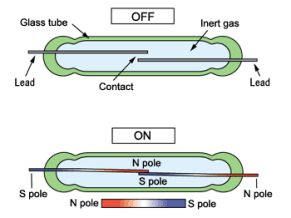
\includegraphics[width=0.5\textwidth]{figuras/reed}
  \caption{\emph{Reed Switch}.}\label{fig:reed}
\end{figure}

O \emph{reed switch} é bem mais barato que o Hall, mas tem pouca durabilidade e elevado tempo de resposta.

\subsection{Chaves de processo}

Chaves de processo são chaves elétricas que atuam quando uma grandeza do processo de fabricação (uma variável de processo) passa determinado nível. Por exemplo: temperatura do tanque 1 acima de \SI{100}{\celsius}, nível do silo abaixo de \SI{2}{\meter}, e assim por diante.

São exemplos de chaves de processo:
\begin{description}
  \item[bóias] que acionam um contato elétrico,
  \item[sensor capacitivo] acionado pelo nível de água de um reservatório,
  \item[chaves de fluxo] onde uma lingueta aciona uma chave eletromecânica se o fluxo passar de um  determinado limite,
  \item[termostatos] que acionam quando a temperatura passa de determinado nível, entre outros.
\end{description}

É cada vez mais comum trocar as chaves de processo por sensores contínuos e implementar o limite de chaveamento no nível de controle da pirâmide. Isto permite uma maior flexibilidade, pois variar o limite no software é mais simples.

\section{Sensores Contínuos}

\subsection{Temperatura}
Entre as diversas maneiras de medir temperatura, destacam-se:
\begin{description}
  \item[Tubo capilar], também conhecido como termômetro líquido. Usa um líquido que ao sofrer expansão térmica ocupa um tubo capilar, que permite visualizar a temperatura. Bom para visualização mas não adequado para automação, por não sr fácil gerar um sinal elétrico a partir dele.

  \item[$\DeltaV_{BE}$] -- pode-se usar dois transistores bipolares para gerar uma diferença de tensão ($\DeltaV_{BE}$) que é proporcional à temperatura absoluta (em Kelvin). É limitado à faixa de temperatura em que a eletrônica funciona: de aproximadamente \SI{-55}{\celsius} a \SI{120}{\celsius}.

  O grande uso da eletrônica fez com que o custo deste tipo de dispositivo caísse bastante, principalmente quando integrado em algum outro circuito. É muito usado em termômetros digitais e no controle de temperatura de processadores de computador.

  \item[Termopar] Pode-se determinar a energia necessária para retirar elétrons de um determinado camada, o que se chama de \emph{função trabalho} do material. Quando dois materiais diferentes se juntam, a diferença da função trabalho deles gera um potencial elétrico. Normalmente este potencial elétrico não é percebido pois ao se fazer um circuito fechado de diferentes materiais com todas as junções na mesma temperatura, estas diferenças acabam se anulando. Porém, se pegarmos dois fios condutores com diferentes funções trabalhos,unirmos uma ponta e colocarmos esta junção numa temperatura diferente, como num forno, por exemplo, aparece uma tensão que é função dos materiais usados e da diferença de temperatura. Este é o chamado efeito Seebeck:
  \[
E = (S_\mathrm{B} - S_\mathrm{A}) \cdot (T_2 - T_1),
  \]
  onde E é a tensão gerada, $S_\mathrm{A}$ e $S_\mathrm{B}$ são os coeficientes de Seebeck dos materiais A e B e $T_2$ e $T_1$ são as diferentes temperaturas.

Logo o termopar mede a diferença de temperatura entre dois lugares e não a temperatura absoluta., precisando de um medidor auxiliar para medir a temperatura ambiente.

Existem diversos tipos de termopar, formados por diferentes junções de metais. Há vários tipos padrões identificados por uma letra: J - ferro e constantan; K - Níquel-Cromo e Níquel-Alumínio; S - Platina e Ródio e Platina. Escolhe-se o tipo pela faixa de operação, precisão e custo.

  \item[Termorresistor] utiliza a variação da resistência de um condutor com a temperatura. Usa um polinômio que relaciona a resistência com a temperatura, como:
  \[
R = R_0[1+a\cdot T+b\cdot T^2],
  \]
onde T é a temperatura em Celsius e $R_0$ é a resistência quando a temperatura é de \SI{0}{\celsius}.

São usados metais inertes, tais como o níquel ou a platina. O nome do sensor é o símbolo do elemento químico usado seguido da resistência à \SI{0}{\celsius}: Pt100, Ni500, etc.
  \item[Pirômetro] ou termômetro de infravermelho usa a chamada raiação do corpo negro para determinar a temperatura. Todo objeto emite fótons de comprimento de onda relacionado à temperatura do objeto. O pirômetro mede então o comprimento de onda destes fótons, permitindo a medição da temperatura à distância.

  Apesar da praticidade ainda são bastante caros. Hoje se usa também as câmeras térmicas, baseadas no mesmo princípio.
\end{description}

\section{Transmissão de dados, aterramento e blindagem em instrumentação.}
